
%----------------------------------------------------------------------------------------
%	PACKAGES AND DOCUMENT CONFIGURATIONS BY DANIEL HEDIGER
%----------------------------------------------------------------------------------------

\documentclass{article}

\usepackage[version=3]{mhchem} % Package for chemical equation typesetting
\usepackage{siunitx} % Provides the \SI{}{} and \si{} command for typesetting SI units
\usepackage{graphicx} % Required for the inclusion of images
\usepackage{natbib} % Required to change bibliography style to APA
\usepackage{amsmath} % Required for some math elements 
\usepackage{german}
\usepackage{float}
\restylefloat{figure}
\usepackage[utf8]{inputenc}
\setlength\parindent{0pt} % Removes all indentation from paragraphs
\renewcommand{\labelenumi}{\alph{enumi}.} % Make numbering in the enumerate environment by letter rather than number (e.g. section 6)

%\usepackage{times} % Uncomment to use the Times New Roman font

%----------------------------------------------------------------------------------------
%	DOCUMENT INFORMATION
%----------------------------------------------------------------------------------------

\title{Physiklabor \\ Laborbericht \\ Wärme} % Title

\author{Daniel \textsc{Hediger} \\ Lucien \textsc{Egloff}} % Author name



\date{\today} % Date for the report

\begin{document}

\maketitle % Insert the title, author and date

\begin{center}
\begin{tabular}{l r}
Ausführungsdatum: & September 12, 2016 \\ % Date the experiment was performed
Dozent: & Dr.Ackermann % Instructor/supervisor

\end{tabular}
\end{center}
\newpage
\tableofcontents 

%----------------------------------------------------------------------------------------
%	SECTION 1
%----------------------------------------------------------------------------------------
\newpage
\section{Aufgabe 1}
Die spezifische Wärmekapazität einer Pfanne soll experimentell bestimmt werden.
\subsection{Grundlagen}
Die Wärmekapazität gibt an wie viel Energie benötigt wird um ein Kilogramm eines Materials um 1 Kelvin zu erhöhen.
Bei homogenen Körpern lässt sich die Wärmekapazität als Produkt der Masse des Körpers und der spezifischen Wärmekapazität berechnen.
\subsection{Resultate}
In dem idealisiert Versuch wird davon ausgegangen das keinen Wärmeaustausch über die Luft stattfindet.Um die Wärmekapazität der Pfanne zu bestimmen wurde die Mischtemperatur berechnet sowie auch gemessen. Da in diesem System die Energieerhaltung gilt, muss die Energiedifferenz die benötigte Energie sein um die Pfanne zu erwärmen.

Unter der Bedingung, dass keine Aggregatzustandsänderung auftritt und das System aus den Körpern abgeschlossen ist gilt:

\begin{equation}
\begin{split}
 Q_{abgegeben} = Q_{aufgenommen}\hspace{0.655cm}\\
 m_1\cdot c_1\cdot (T_1-T_m)=m_2\cdot c_2\cdot (T_2-T_m)
\end{split}
\end{equation}
Die aufgelöste Formel nach der Mischungstemperatur:
\begin{equation}
	T_m = \frac{m_1\cdot c_1\cdot T_1+m_2\cdot c_2\cdot T_2}{m_1\cdot c_1+m_2\cdot c_2}
\end{equation}
Aus der Mischtemperatur$(T_{mberechnet})$ und Mischtemperatur$(T_{mgemessen})$ kann die Wärme $Q$ berechnet werden, welche in die Pfanne übergegangen ist.
\begin{equation}
 Q = (m_{w1}+m_{w2}) \cdot c_w \cdot (T_m{berechnet}-T_m{gemessen})
\end{equation}
Somit kann die spezifische Wärmekapazität berechnet werden mit :
\begin{equation}
	c_{Pfanne} = \frac{Q}{m_{Pfanne} \cdot (T_{p1}-T_{p2}) }
\end{equation}


\newpage
\textbf{Beschreibung Tabelle}

  \begin{description}
    \item[\textbf{ $Tw_k$}]= Temperatur des kalten Wasser in $[C^\circ]$
    \item[\textbf{ $Tw_w$}]= Temperatur des warmen Wasser in $[C^\circ]$
    \item[\textbf{ $mw_k$}]= Masse des kalten Wasser in $[g]$
    \item[\textbf{ $mw_w$}]= Masse des warmen Wasser in $[g]$
    \item[\textbf{ $Tm_g$}]= Gemessene Temperatur des Mischwasser in  $[C^\circ]$
    \item[\textbf{ $Tm_g$}]= Berechnete Temperatur des Mischwasser in  $[C^\circ]$
    \item[\textbf{ $c$}]=  Berechnete spez. Wärmekapazität  $[\frac{Kg}{J \cdot K}]$
    
  \end{description}
\begin{table}[h]
    \begin{tabular}{|l|l|l|l|l|l|l|l|}
    
        \hline
        Durchgang &\textbf{$Tw_k$} &\textbf{$Tw_w$}& \textbf{$mw_k$}&\textbf{$mw_w$}&\textbf{$Tm_g$}&\textbf{$Tm_b$}&\textbf{$c$}\\ \hline
        1         & 18.6 & 55 & 645& 276 & 31.8 &29.5&657.83\\ 
        2         & 18.2 & 63 &500 &240  & 38 &42.73&651.23\\ 
        3         & 16 & 69 &659 &497  &41 &36.73&805.43\\ 
        4         &  18.2  &50 & 780 & 709 &33&33.74&305.02\\ \hline
        \textbf{Mittelwert} &\textbf{17.75}&\textbf{59.25}&\textbf{646}  &\textbf{430.5}  &\textbf{37.45} &\textbf{33.18}&\textbf{604.88} \\ 
        \hline
    \end{tabular}
\end{table}

\subsection*{Schlussfolgerung}
Gemäss schweizer-fn.de beträgt die spez. Wärmekapazität von Chromstahl 457$[\frac{Kg}{J \cdot K}]$, unser Wert liegt bei 604.88 $[\frac{Kg}{J \cdot K}]$ und somit ist das gemessene Resultat plausibel. Die Abweichung hat folgende Gründe:\\
\textbf{a)} Verluste durch äussere Einflüsse wurden vernachlässigt.\\
\textbf{b)} Die Dauer des Versuches musste klein gehalten werden damit nicht zu viele Verluste entstehen. Idealerweise müsste länger gewartet werden bis sich das System einpendelt.

\section{Versuch 2}
Bestimmen Sie die spezifische Schmelzwärme von Eis indem Sie Eis in die mit Wasser gefüllte Pfanne geben.
Halten Sie die Wassertemperatur als Funktion der Zeit in einem Diagramm fest. Führen Sie das Experiment
mit einem grossen Eisklotz und mit zerdrücktem Eis durch.
\subsection{Grundlage}
Bei diesem Versuch wurde bei einer bestimmten Menge Wasser und bestimmter Anfangstemperatur 
Eis dazugegeben. Es gilt die Temperaturänderung des Wassers in Funktion der Zeit aufzuzeigen. 
Dabei gilt es eine angemessene Anfangstemperatur des Wassers festzulegen um sicherzustellen, dass 
der Schmelzversuch nicht zu langsam aber auch nicht zu schnell von statten geht. Doch vorerst 
mussten folgende Messwerte ermittelt werden
\subsection{Resultate}
Zuerst wurde die Energiebilanz aufgestellt:
\begin{equation}
Q_{Wasser}+Q_{Pfanne}+Q_{Eiswasser} = Q_{Wasser}+Q_{Eis}-Q_{Schmelz}+Q_{Panne}
\end{equation}
Daraus folgt:
\begin{equation}
(m_{w}+m_{ew})\cdot c_{w}\cdot T_m+m_{p}\cdot c_{p}\cdot T_m= \\ m_{w} \cdot c_{w} \cdot T_{w}+ m_{e} \cdot c_{w} \cdot T_{0^\circ}-Q \cdot m_{e}+m_{p} \cdot c_{p} \cdot
 T_{p}
\end{equation}

Die Formal nach $Q_{Schmelz}$ umgeformt:

\begin{equation}
c_{s} = \frac{T_{w}(m_{w} \cdot c_{w}+m_{p} \cdot c_{p})-T_{m}((m_{w}+m_{e}) \cdot c_{w}+m_{p} \cdot c_{p})}{m_{e}}
\end{equation}
\subsubsection{Gemessene Grössen}
  \begin{description}
    \item[\textbf{ $Tw_1$}]= Temperatur des Wasser bei Eisklotz vorher= 53.7$[C^\circ]$ 
        \item[\textbf{ $Tw_1$}]= Temperatur des Wasser bei Eisklotz nachher= 38.5.7$[C^\circ]$ 
     \item[\textbf{ $Tw_2$}]= Temperatur des Wasser des zerdrückten Eis vorher =  15.3 $[C^\circ]$ 
          \item[\textbf{ $Tw_2$}]= Temperatur des Wasser des zerdrückten Eis nachher =  0.9 $[C^\circ]$ 
    \item[\textbf{ $m_w$}]= Masse des Wasser 1 $[kg]$
     \item[\textbf{ $m_k$}]= Masse des Eisklotzes 0.16 $[kg]$
    \item[\textbf{ $m_z$}]= Masse des zerdrückten Eis 0.287 $[kg]$
      \item[\textbf{ $m_p$}]= Masse Pfanne 1.021 s$[kg]$
  \end{description}
 \textbf{Berechnung Eisklotz}\\
 Aus Formel (7) ergibt sich:
 \begin{equation}
 \tfrac{53.7 \cdot (4180+1.021 \cdot 604.66)-38.5\cdot (1.21+1+4180+1.021 \cdot 604.66)}{0.16} = \underline{\underline{454.963kJ \cdot kg^-1}} 
 \end{equation}  
 
  \textbf{Berechnung zerdrücktes Eis}\\
  \begin{equation}
 \tfrac{15.3 \cdot (4180+1.021 \cdot 604.66)-0.9\cdot (1.21+1+4180+1.021 \cdot 604.66)}{0.287} = \underline{\underline{340.704kJ \cdot kg^-1}} 
 \end{equation}  
 
 \subsubsection{Grafik zur Messung}
 \begin{figure}[H]
\includegraphics[scale=0.7]{EK.pdf} 
\caption{Messwerte Eisklotz.}
\end{figure}
 \begin{figure}[H]
\includegraphics[scale=0.7]{ZE.pdf} 
\caption{Messwerte zerdrücktes Eis.}
\end{figure}

\subsection{Schlussfolgerung}
Gemäss Tabelle aus dem Taschenbuch der Physik von Horst Kuchling S.636 beträgt der Wert der 
Schmelzwärme von Eis 334kJ/kg.  
Da es sich bei diesem Versuch um Zerdrücktes Eis und dieses eine viel grössere Fläche gegenüber 
dem Wasser ergibt, wird das Resultat viel genauer.
\section{Versuch 3}
Wasser wurde auf einem Gaskocher zum Kochen gebracht. Der 
Temperaturverlauf wurde als Funktion der Zeit festgehalten. Damit soll bestimmt werden, was für ein 
Wirkungsgrad das Erwärmen von Wasser hat und ob man ihn mit einem Deckel verbessern kann.  
\subsection{Versuchsaufbau}
\begin{figure}[H]
\begin{center}
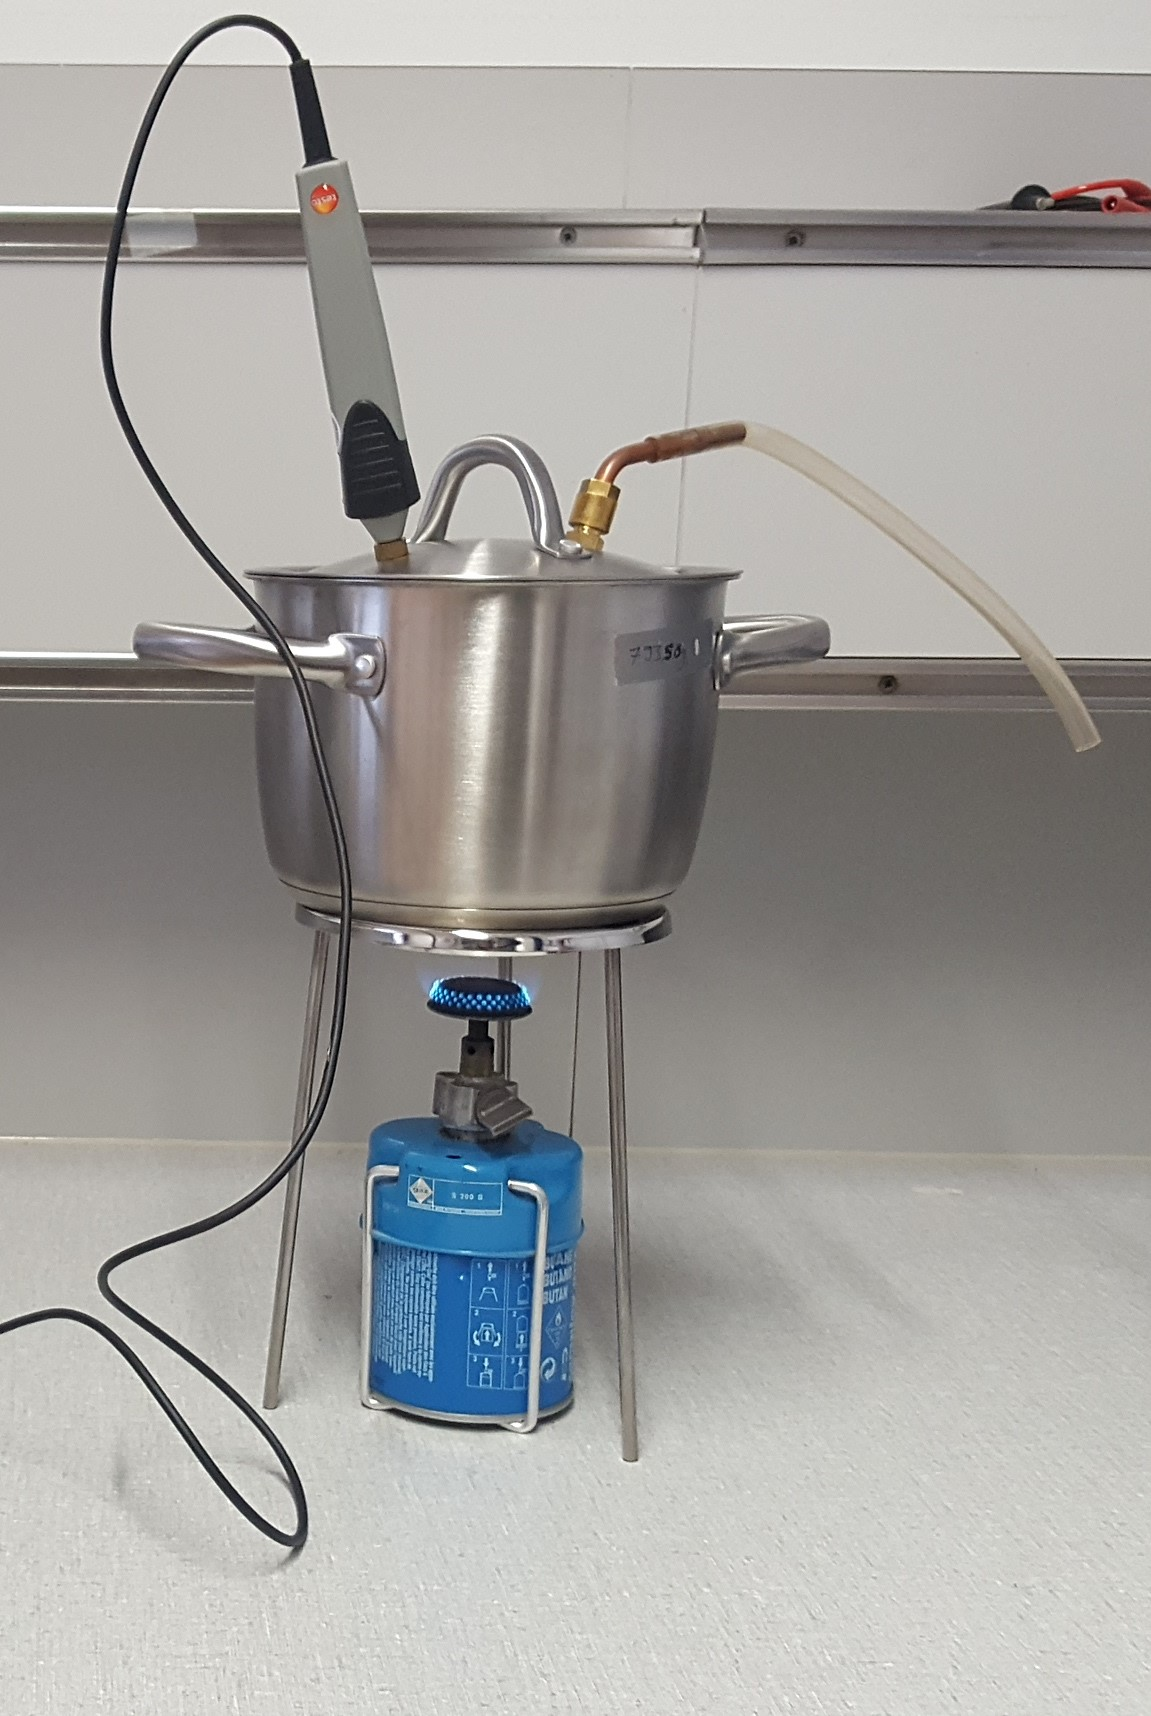
\includegraphics[scale=0.3]{Waerme1.pdf} 
\caption{Wasser wird über dem Gaskocher erhitzt.}
\end{center}
\end{figure}
\subsection{Resultate}
Da das Wasser mit einem Gaskocher erhitzt wurde, muss die Zugeführte Energie wie folgt berechnet werden:
\begin{equation}
 Q_{Zugefuehrt} = \Delta m \cdot H_s
\end{equation}
Wobei $H_s$ der Brennwet von Propangas ist.\\\\
\textbf{Ohne Deckel}
\begin{equation}
P_{Zugefuehrt} = \frac{Q_{Gas}}{t} = \frac{0.0198Kg\cdot k0.33MJ \cdot kg^-1}{780sek} = \underline{1219.53 W }
\end{equation}
\begin{align}
\begin{split}
P_{w} = \frac{Q_w}{t} = \frac{m_{w} \cdot c_{w} \cdot \Delta T}{t}=  \frac{1kg \cdot 4180 \cdot (80C^\circ-18.4C^\circ)}{780sek} = \underline{330.11W}
\end{split}
\end{align}

\begin{equation}
\eta = \frac{P_{Wasser}}{P_{Zugefuehrt}} = \underline{0.271}\Rightarrow \underline{\underline{27.1\%}}
\end{equation}
\textbf{Mit Deckel}
\begin{equation}
P_{Zugefuehrt} = \frac{Q_{Gas}}{t} = \frac{0.0198Kg\cdot 50.33MJ \cdot Kg^-1}{630sek} = \underline{1509.9 W }
\end{equation}
\begin{align}
\begin{split}
P_{w} = \frac{Q_w}{t} = \frac{m_{w} \cdot c_{w} \cdot \Delta T}{t}=  \frac{1kg \cdot 4180 \cdot (80-17.0)}{630sek} = \underline{418W}
\end{split}
\end{align}
\begin{equation}
\eta = \frac{P_{Wasser}}{P_{Zugefuehrt}} = \underline{0.277}\Rightarrow \underline{\underline{27.7\%}}
\end{equation}
\begin{figure}[H]
\includegraphics[scale=0.5]{Waerme.pdf} 
\caption{Vergleich mit und ohne Deckel.}
\end{figure}


\subsection{Schlussfolgerung}
Die Zugeführte Energie wurde nicht ausschliesslich zum Erwärmen des Wassers verwendet. Der Schlecht Wirkungsgrad entsteht durch schlecht Zuführung der Wärme, weil der Brenner hohe Verluste verursacht. Dadurch wird die Prognose das wird ein höheren Wirkungsgrad mit dem Deckel haben nicht mehr deutlich sichtbar. Bessere Resultate sind erzielbar durch verwenden einer Herdplatte.
\section{Versuch 4}
Die spezifische Verdampfungs‐ bez. Kondensationswärme soll bestimmt werden, indem der Wasserdampf in eine
mit Wasser gefüllte Pfanne geführt wird.
\subsection{Grundlage}
Bei diesem Versuch soll eine gewisse Menge Wasser in einem Isolierten Kochtopf mittels der 
Dampfwärme aus einem anderen Kochtopf erwärmt werden. Der Kochtopf und das zu erwärmende 
Wasser im Isoliertopf sind über ein kleines Röhrensystem miteinander verbunden. Dabei soll der 
Temperaturverlauf des zu erwärmenden Wassers sowie die Gewichtsveränderung gemessen werden. 
\subsection{Versuchsaufbau}
\begin{figure}[H]
\includegraphics[scale=0.5]{Pot.pdf} 
\caption{Durch verdampfen und wider kondensieren soll Energie von dem rechten in den linken Topf gelangen.}
\end{figure}
\subsection{Resultate}

\begin{tabular}[H]{l r}
$m_p$ Masse der Pfanne & 1.023 Kg \\
$m_1$ Anfangsmasse der Pfanne & 1.050 Kg \\
$m_2$ Endmasse der Pfanne &  1.079 Kg \\
$T_1$ Anfangstemperatur & 16.8 $C^\circ$ \\
$T_2$ Endtemperatur & 37.0 $C^\circ$ \\
$T_d$ Dampftemperatur & 100 $C^\circ$ 

\end{tabular}

\subsubsection{Auswertung}
Masse des zugeführten Dampfes:
\begin{equation}
m_d = m_2 - m_1 = 1.079kg - 1.050 kg = \underline{29g}  
\end{equation}
Durch Energiegleichsetzung erfolgt :
\begin{equation}
Q_{Wasser1}+Q_{Dampf}+Q_{Verdampfung}+Q_{Pfanne} = Q_{w2}+Q_{v}+Q_{p}
\end{equation}
\begin{equation}
c_{d} = \frac{T_2 \cdot c_w \cdot(m_w+m_d)+T_2\cdot c_p \cdot m_p -c_w \cdot (m_{w1}\cdot T_1 + m_d \cdot T_d)+T_1 \cdot m_p \cdot c_p}{m_d}
\end{equation}
Ausgewertet bedeutet das:
\begin{equation}
\underline{\underline{2.499 MJ \cdot kg^-1}}
\end{equation}

\subsection{Schlussfolgerung}
Der richtige Wert liegt bei 2.2 $\frac{MJ}{Kg}$. Diese Abweichung lässt sich erklären das auch Dampf an die Umgebung abgegeben wird welche nicht berücksichtigt werden kann.  
\end{document}